% Robosim Programmer's Guide
% ============================
% Gustavo Muñoz
% December 3rd, 2022

\documentclass[12pt,a4paper,oneside,english]{book}

\usepackage[english]{babel}
\usepackage[latin1]{inputenc}
\usepackage[a4paper,left=3cm,right=3cm,top=3.5cm,bottom=3.5cm]{geometry}
\usepackage[doublespacing]{setspace}
\usepackage{color}
\usepackage{hyperref}
\usepackage{fancyhdr}
\usepackage{amsmath}
\usepackage{graphicx}
\usepackage{array}
\usepackage{afterpage}
\usepackage{amsfonts}
\usepackage{indentfirst}
\usepackage{amssymb}
\usepackage{verbatim}

\pagestyle{fancy}
\headheight 15pt

%%%%%%%%%%%%%%%%%%%%%%%%%%%%%%%%%%%%
%     To modify the cover page     %
%%%%%%%%%%%%%%%%%%%%%%%%%%%%%%%%%%%%

% TOP
\fancyhead[L]{Robosim Programmer's Guide}
\fancyhead[R]{\thesection}

% BOTTOM
\fancyfoot[L]{Gustavo Mu\~{n}oz}
\fancyfoot[C]{\thepage}
\fancyfoot[R]{Therian Corp.}
\renewcommand{\footrulewidth}{1pt}

\begin{document}
\frontmatter

%%%%%%%%%%%%%%%%%%%%%
%     Title Page    %
%%%%%%%%%%%%%%%%%%%%%

\begin{titlepage}

  \begin{figure}[h]  % Logo %
    \begin{center}
      
\includegraphics[width=0.30\textwidth]{images/Logo.png}
    \end{center}
  \end{figure}

  \vspace{5mm}
  \begin{center}
    \Huge
    Robosim Programmer's Guide
  \end{center}

  \vspace{20mm}
  \begin{center}
    Gustavo Mu\~{n}oz
  \end{center}

\end{titlepage}

% Here we have the special sections of the document
\tableofcontents
\listoffigures
\listoftables

%%%%%%%%%%%%%%%%%%%%%%%%
%     Introduction     %
%%%%%%%%%%%%%%%%%%%%%%%%

\chapter{Introduction}

Robosim project has been design to cover a few aspects of robotic design and robotic behavior algorithms. And for me, to learn Java and OpenGL, and to improve my skills in fuzzy logic and robotic design (cinematic and dynamics).

I'm trying to develop a 3D environment to work with robotics and to create 3D objects and mathematic tools to manipulate them. The program is very simple and the GUI allow us to work from code. We can add as many GUI elements as we need, and of course more GLCanvas to render other views or even other environments.

If you respect the main structure of the basic 3D Object, making new objects is as simple as creating new classes and importing them into the NetBeans project. You can make them as complex as you want, and draw your experiment including the new field containing your 3D objects and algorithms into the drawing chain. The concept of the program/project is shown in Figure \ref{full program structure}. Is very powerful because you can do whatever you want and you only are limited by code and your knowledge of Java and OpenGL, and there is no restrictions by my side except basic program structure to automatize the drawing process.

\begin{figure}[htbp]
  \begin{center}
    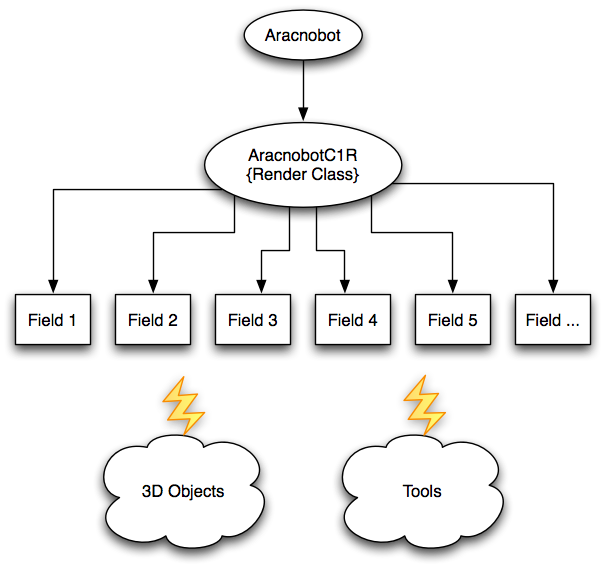
\includegraphics[width=1.0\textwidth]{images/FPS.png}
    \caption{Full Program Structure}
    \label{full program structure}
  \end{center}
\end{figure}

%%%%%%%%%%%%%%%%%%%%
%     Document     %
%%%%%%%%%%%%%%%%%%%%

\mainmatter

% FIRST PART

\part{Robosim Project GUI}

\chapter{An Overview of the GUI}

The Robosim Project GUI is a Java application that contains a big GLCanvas to draw an OpenGL scene where the robots are going to be drawn. The interesting thing of Robosim is that is a visual project, and that means, we are going to be able to draw all the code results.

The environment consist on a main class that implements all the objects we are going to draw in its constructor and then we are going to be able to modify the objects parameters using the drawing thread or the mouse and keyboards events. And of course, being a JFrame allows us to include objects such as slider or buttons to interact with our environment.

\chapter{Objects}

\section{Point3D}

Point3D is a class that allows us to have a point in our 3D space with different data types inside and different coordinate system representations. We are going to have the point in this ways:

\begin{enumerate}
  \item Rectangular Coordinates.
  \item Polar Coordinates.
  \item Cylindrical Coordinates.
  \item Spherical Coordinates.
  \item Point3d.
  \item Vector3d.
\end{enumerate}

\newpage

\subsection{Rectangular Coordinates}

The most common representation to operate between points in our space. We need this representation only for mathematics. We are going to use more intuitive representations to define components but to operate we need to do it in rectangular coordinates. The components of this system are $\left\{X,Y,Z\right\}$  as you can see in Figure \ref{rectangular coordinates}.

\begin{figure}[htbp]
  \begin{center}
    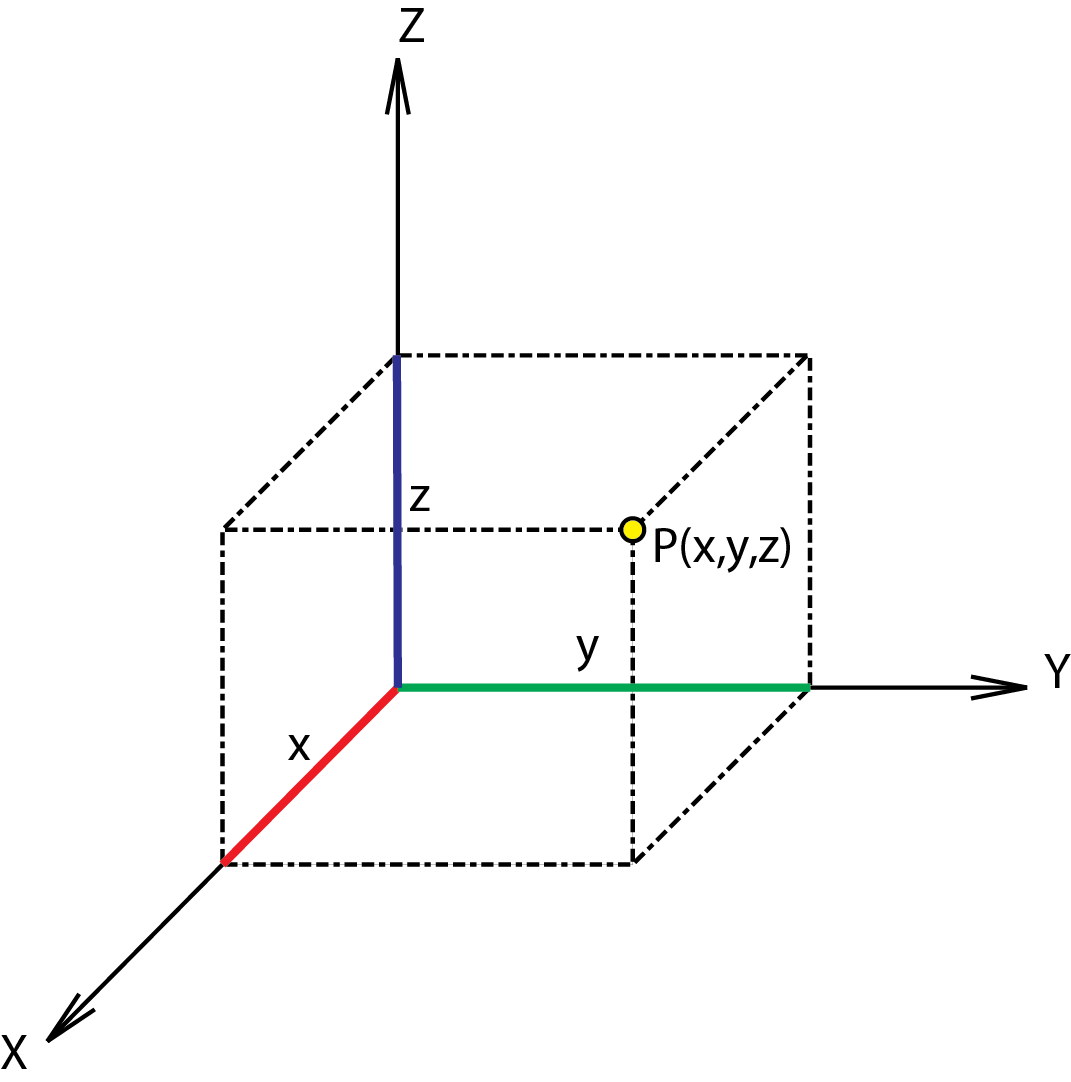
\includegraphics[width=0.50\textwidth]{images/RC.png}
    \caption{Rectangular Coordinates}
    \label{rectangular coordinates}
  \end{center}
\end{figure}

\newpage

\subsection{Polar Coordinates}

Polar coordinates are the first step for the others coordinate systems. They are the projection in XY plane of cylindrical coordinates, or spherical coordinates with a $\phi$ angle of 90 degrees. The components of this system are $\left\{\rho,\theta\right\}$ as you can see in Figure \ref{polar coordinates}. To transform to rectangular coordinates, we use the following equations:

\begin{itemize}
  \item $x=\rho\cdot\cos(\theta)$
  \item $y=\rho\cdot\sin(\theta)$
\end{itemize}

\begin{figure}[htbp]
  \begin{center}
    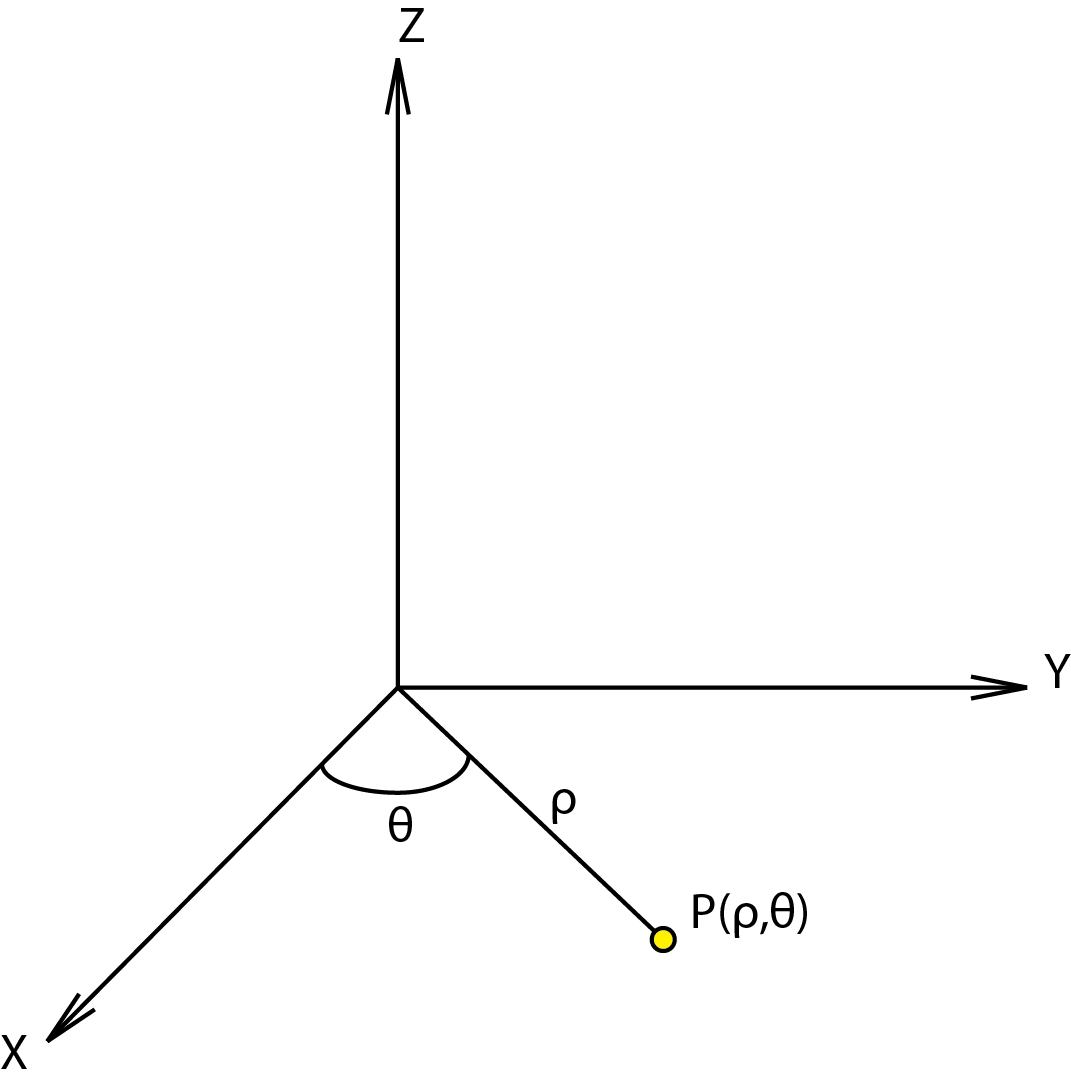
\includegraphics[width=0.50\textwidth]{images/PC.png}
    \caption{Polar Coordinates}
    \label{polar coordinates}
  \end{center}
\end{figure}

\newpage

\subsection{Cylindrical Coordinates}

Cylindrical coordinates are similar to polar coordinates but with a height along the Z axis. To transform them into rectangular coordinates, we use the following equations:

\begin{itemize}
  \item $x=\rho'\cdot\cos(\theta)$
  \item $y=\rho'\cdot\sin(\theta)$
  \item $z=z$
\end{itemize}

$\rho'$ is the projection of the $\rho$ vector on XY, or the $\rho$ vector with height $z$ equal to zero.

\begin{figure}[htbp]
  \begin{center}
    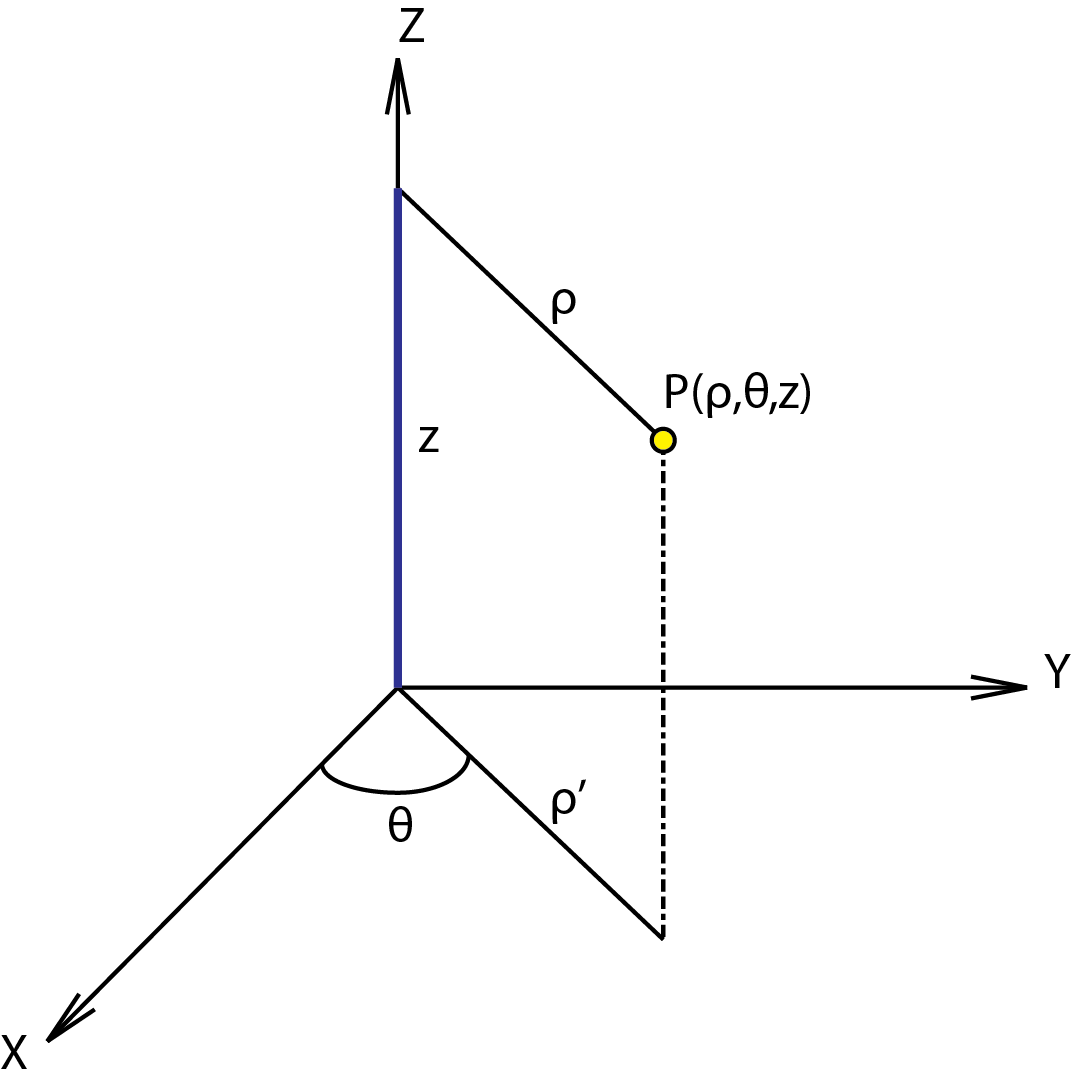
\includegraphics[width=0.50\textwidth]{images/CC.png}
    \caption{Cylindrical Coordinates}
    \label{cylindrical coordinates}
  \end{center}
\end{figure}

\newpage

\subsection{Spherical Coordinates}

Spherical coordinates are the most intuitive reference system to work in 3D. If we use them to define a position or a speed, the reference to the coordinate origin is an amount we can interpret for example as 3 m or 2.5 m/s. To modify the position in space is as easy as modify two angles, and always working with positive values. This makes programming easier than with other reference systems. To obtain rectangular coordinates we need the following equations:

\begin{itemize}
  \item $\rho'=\rho\cdot\sin(\phi)$
  \item $x=\rho'\cdot\cos(\theta)=\rho\cdot\sin(\phi)\cdot\cos(\theta)$
  \item $y=\rho'\cdot\sin(\theta)=\rho\cdot\sin(\phi)\cdot\sin(\theta)$
  \item $z=\rho\cdot\cos(\phi)$
\end{itemize}

\begin{figure}[htbp]
  \begin{center}
    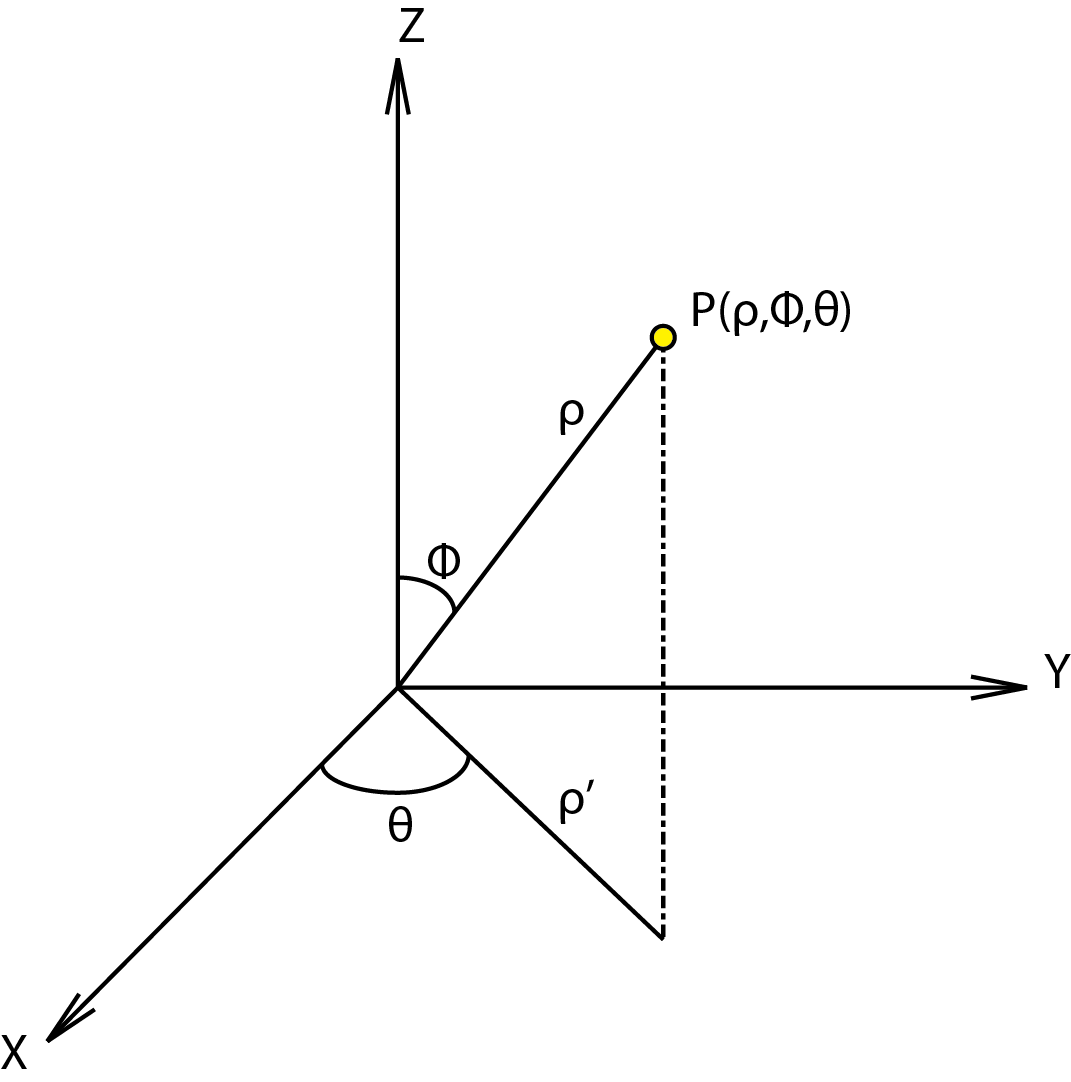
\includegraphics[width=0.50\textwidth]{images/SC.png}
    \caption{Spherical Coordinates}
    \label{spherical coordinates}
  \end{center}
\end{figure}

\newpage

\subsection{Point3d}

Here we are going to start using Java 3D API variable types. Point3d is basically what its names sows; a point defined using tree doubles. We need this data type to transform our Point3D using homogeneous transformation matrices. The fourth element for the transformation is automatically set to 1, and the new transformed coordinates are stored in our point, inside the Point3D structure.

\subsection{Vector3d}

We need this data type to be able to use our Point3D as a vector and transform it using vector mathematics and operations like vector addition, dot product, cross product$\dots$

\section{Object3D}

The Object3D is the next link in our chain to draw in the scene. This is the basic element inside the scene and contains two Point3D objects for position and speed, and a virtual function to draw the object into the scene. Of course every Object3D has its own identifier string \textbf{id} to define what are we drawing, and every descending class should implements its own display function. In other case we are going to have a error. There is no Object3D without a graphic output.

\section{Axis}

Axis is the class we use when we need to draw an axis object. We can place this object everywhere into the scene and define the labels we are going to put on the axis and the length of the axis.

\section{Grid}

This is a simple grid to use as reference for a surface, for example the floor or the roof of our scene. There is no interaction with it and is invisible for the elements into our 3D space.

\section{Text3D}

If we need to write something on screen we use this function to write it. Its a very simple class that extends Object3D and receive a position in space and a string to plot.

\section{OGLColor}

Here we can define colors and materials for the objects into the scene. There are plain objects as points and lines that only have color, and others that can have texture. We need to distinguish between them because lights only affect the object with materials. When we want to draw a plain object, we need to turn of the lights.

\begin{verbatim}
\end{verbatim}

\section{Robot}

This basically is a red cylinder we move around our room where we have the obstacles. The robot use the collision solver class to avoid obstacles and bounce against walls.

\section{Obstacle}

The obstacles are blue cylinders we use to make robots avoid them. The speed vector for obstacles is zero, so only robots have movement into the scene. To create them we use \textbf{Math.random()} function and we modify for each obstacle the distance to the origin and the angle with the $X$ axis. All the objects in our collision field are on the $XY$ plane.

\section{Wall}

A simple 3D wall we can place wherever we want. Of course we can set its dimensions and we can use them as borders or as obstacles inside our field of play. A nice experiment could be to build a labyrinth and to put a robot inside to bounce against walls till it leaves the labyrinth.

\section{Denavit-Hartenberg Robots}

Denavit-Hartenberg is an standard in industry. When you want to define dimensions and dof of a robot (degrees of freedom) you use DH parameters. Each joint into a robot has four parameters that correspond to standard transformations to go from one joint to the next one in the cinematic chain. The four parameters are:

\begin{description}
  \item[$\theta$ ] Is a rotation around $Z$ axis to make $X$ axis coincident.
  \item[d ] Is a translation along the $Z$ axis until the center of our two coordinates systems are coincident along the $X$ axis.
  \item[a ] Is a translation along the $X$ axis to make centers coincident.
  \item[$\alpha$ ] Is a rotation around $X$ axis to make $Z$ axis coincident.
\end{description}

We choose $Z$ axis along the movement of the joint (rotation axis or translation direction). The $X$ axis is perpendicular to booth $Z$ axis (joint \textbf{i} and joint \textbf{i+1}) and the $Y$ axis is according to axis rules. You can see the parameters in the Figure \ref{dh parameters}. An example of the DH parameters for a commercial robot are shown in Table \ref{irb6400c dh parameters}. These are the parameters for a ABB IRB6400C. You can create a new field to draw it and pass the DHRobot constructor the DH parameters matrix for this robot.

\begin{figure}[htbp]
  \begin{center}
    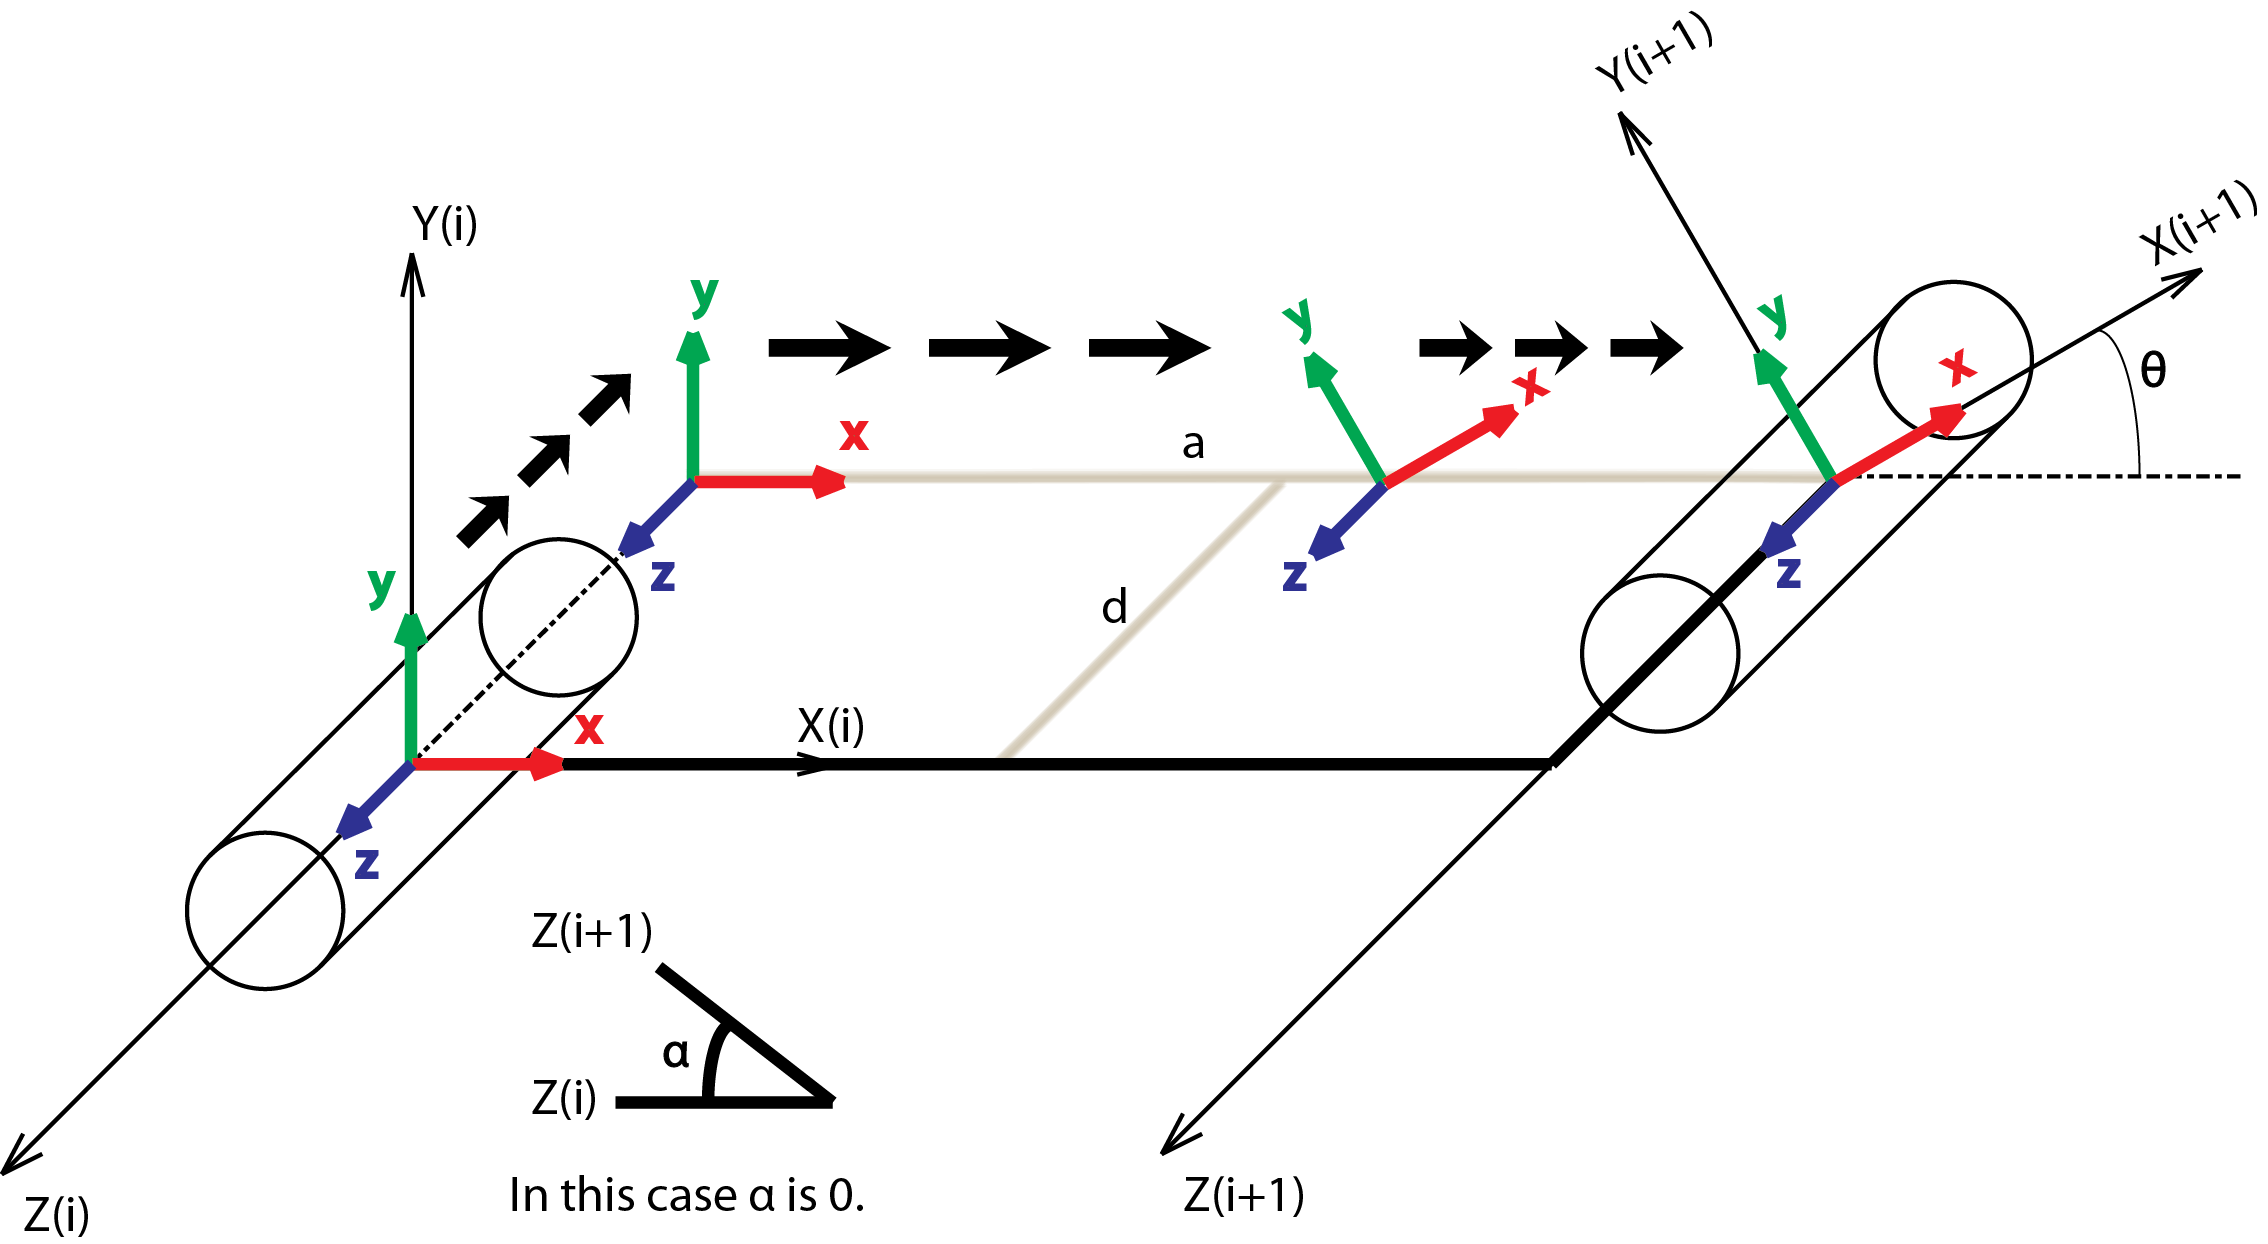
\includegraphics[width=1.0\textwidth]{images/DHP.png}
    \caption{Denavit-Hartenberg Parameters}
    \label{dh parameters}
  \end{center}
\end{figure}

\begin{table}[htp]
  \caption{IRB6400C DH Parameters}
  \begin{center}
    \begin{tabular}{|m{1cm}|>{\centering\arraybackslash}m{1.5cm}|>{\centering\arraybackslash}m{1.5cm}|>{\centering\arraybackslash}m{1.5cm}|>{\centering\arraybackslash}m{1.5cm}|}
      \hline
      Joint   & $\theta$                & d       & a        & $\alpha$      \\
      \hline
      $J_{1}$ & $\theta_{1}$            & 0       & 0        & $-90^{\circ}$ \\
      \hline
      $J_{2}$ & $\theta_{2}$            & $l_{1}$ & 0        & $90^{\circ}$  \\
      \hline
      $J_{3}$ & $\theta_{3}-90^{\circ}$ & 0       & $-l_{2}$ & $90^{\circ}$  \\
      \hline
      $J_{4}$ & $\theta_{4}$            & $l_{3}$ & 0        & $-90^{\circ}$ \\
      \hline
      $J_{5}$ & $\theta_{5}$            & 0       & 0        & $90^{\circ}$  \\
      \hline
      $J_{6}$ & $\theta_{6}$            & $l_{4}$ & 0        & 0             \\
      \hline
    \end{tabular}
  \end{center}
  \label{irb6400c dh parameters}
\end{table}

When we have all the parameters into a table, we can create a transformation matrix with each row. The full transformation matrix is a compose matrix with four partial transformations that we will se in Chapter \ref{tools}.

\subsection{Joint}

This is basically a sphere in a 3D space. When you create a sphere using GLUT libraries, it appears in coordinates origin so we need to transform the OpenGL scene to move it. I have solve this problem creating a class that draws a sphere and transform it to put in a determinate coordinates in our 3D space.\\

\noindent
\textcolor[rgb]{0.00,0.00,1.00}{public} \textbf{Joint}(\textcolor[rgb]{0.00,0.00,1.00}{double} radius, \textcolor[rgb]{0.00,0.00,1.00}{double} x, \textcolor[rgb]{0.00,0.00,1.00}{double} y, \textcolor[rgb]{0.00,0.00,1.00}{double} z);

\subsection{Link}

A link is a cylinder linking two joints. Of course the problem is that you only can create cylinders in the coordinate origin, so if you want to put a cylinder between two point you have to use OpenGL transformations. I have create a Link class that solves this problem and you only need to pass the initial point and the end point to create the link.\\

\noindent
\textcolor[rgb]{0.00,0.00,1.00}{public} \textbf{Link}(\textcolor[rgb]{0.00,0.00,1.00}{double} x1, \textcolor[rgb]{0.00,0.00,1.00}{double} y1, \textcolor[rgb]{0.00,0.00,1.00}{double} z1, \textcolor[rgb]{0.00,0.00,1.00}{double} x2, \textcolor[rgb]{0.00,0.00,1.00}{double} y2, \textcolor[rgb]{0.00,0.00,1.00}{double} z2)

\subsection{DHRobot}

And finally we are going to create the robot. We need only two basic parameters; the position and speed of the base, and the Denavit-Hartemberg parameter matrix.\\

\noindent
\textcolor[rgb]{0.00,0.00,1.00}{public} \textbf{DHRobot}(\textcolor[rgb]{0.00,0.00,1.00}{double} base[], \textcolor[rgb]{0.00,0.00,1.00}{double} dhmatrix[][])\\

The first parameter is a double array. The first tree elements are the position of the base, and the rest are the speed of the base. This is useful if we want to move the robot around our 3D space.

The second parameter is the DH matrix with the dh parameters for all the joints in the robot. In this matrix are fixed parameters according with the robot structure and variable parameters according with the degrees of freedom of the joints of the robot. Changing this values, we will be able to animate the robot in our scene.

\subsection{DHRobotB1}

This is a robot based in Denavit-Hartenberg algorithms on top ob a base to make it a little more realistic. Just an experiment but nothing mathematically relevant.

\chapter{Tools}
\label{tools}

\section{Introduction}

The mathematics is a mix between OpenGL and Denavit-Hartemberg transformation matrices using the Java 3D API that provides us with methods to use vector mathematics and transformations for points. The important thing is to separate internal transformations from environment transformations.

We are going to transform the global scene with OpenGL transformations to situate our point of view to a $\left\{X,Y,Z\right\}$ normal view, but all the transformations of the objects are made before the scene transformation, so we need to think in the scene original coordinates to create objects and then move all the scene to see it better or even to manipulate through mouse and keyboards events.

\section{Denavit-Hartenberg Transformations}

To create the DH matrix we need to do four transformations. Those transformations are: a rotation $\theta$ around $Z$ axis, a translation d along $Z$ axis, a translation a along $X$ axis and a rotation $\alpha$ around $X$ axis.

$A_{i}^{i-1} = Rot(\theta_{i},z)\cdot Trans(d_{i},z)\cdot Trans(a_{i},x)\cdot Rot(\alpha_{i},x) =$

\[
  \begin{pmatrix}
    c(\theta_{i}) & -s(\theta_{i}) & 0 & 0 \\
    s(\theta_{i}) & c(\theta_{i})  & 0 & 0 \\
    0             & 0              & 1 & 0 \\
    0             & 0              & 0 & 1
  \end{pmatrix}
  \begin{pmatrix}
    1 & 0 & 0 & 0     \\
    0 & 1 & 0 & 0     \\
    0 & 0 & 1 & d_{i} \\
    0 & 0 & 0 & 1
  \end{pmatrix}
  \begin{pmatrix}
    1 & 0 & 0 & a_{i} \\
    0 & 1 & 0 & 0     \\
    0 & 0 & 1 & 0     \\
    0 & 0 & 0 & 1
  \end{pmatrix}
  \begin{pmatrix}
    1 & 0             & 0              & 0 \\
    0 & c(\alpha_{i}) & -s(\alpha_{i}) & 0 \\
    0 & s(\alpha_{i}) & c(\alpha_{i})  & 0 \\
    0 & 0             & 0              & 1
  \end{pmatrix}
  =
\]

\[
  \begin{pmatrix}
    c(\theta_{i}) & -c(\alpha_{i})\cdot s(\theta_{i}) & s(\alpha_{i})\cdot s(\theta_{i})  & a_{i}\cdot c(\theta_{i}) \\
    s(\theta_{i}) & c(\alpha_{i})\cdot c(\theta_{i})  & -s(\alpha_{i})\cdot c(\theta_{i}) & a_{i}\cdot s(\theta_{i}) \\
    0             & s(\alpha_{i})                     & c(\alpha_{i})                     & d_{i}                    \\
    0             & 0                                 & 0                                 & 1
  \end{pmatrix}
\]
\\
We use the matrices to go from the base to the end effector through every joint. We have to do partial steps to know the position of every joint to be able to draw it in our workspace. When we have this defined we only need to repeat this structure for every robot we want to create. if we want to chain different robots we only need to place the base of the new robot at the end of the previous robot. Now, if we move the last robot, we moved the base of the new robot and when we calculate the transformations for the new robot we start from the position of the new base.

\section{Environment Manipulator}

Here we are going to implement all the algorithms to manipulate the point of view for our 3D space. The EnvManipulator object takes the dimension of the screen and the position in $\{x,y\}$ to determine the $\Delta x$ and $\Delta y$ of the mouse movement and the transformation of this increment into a rotation and a translation in OpenGL of the elements of the scene.

\section{Collision Solver}

The collision solver is a class that takes an object in movement, and an array ob possible obstacles, and calculates the action to avoid them. To react to the collision we use fuzzy logic created with Xfuzzy tool as we can see in Figure \ref{position of the obstacle} and Figure \ref{fuzzy system based on collision distance}.

\begin{figure}[htbp]
  \begin{center}
    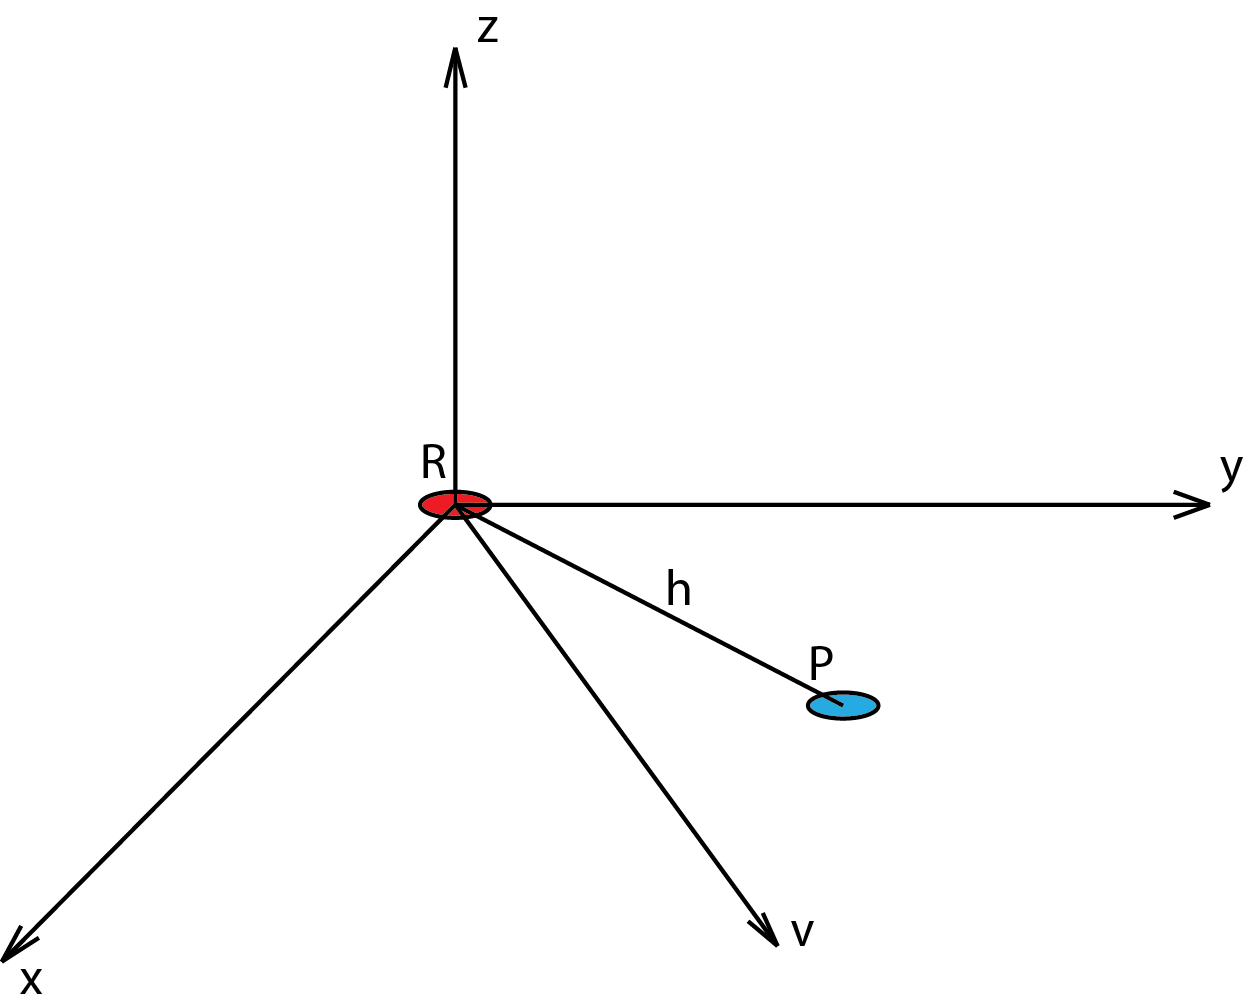
\includegraphics[width=0.5\textwidth]{images/AC01.png}
    \caption{Position of the Obstacle}
    \label{position of the obstacle}
  \end{center}
\end{figure}

\begin{figure}[htbp]
  \begin{center}
    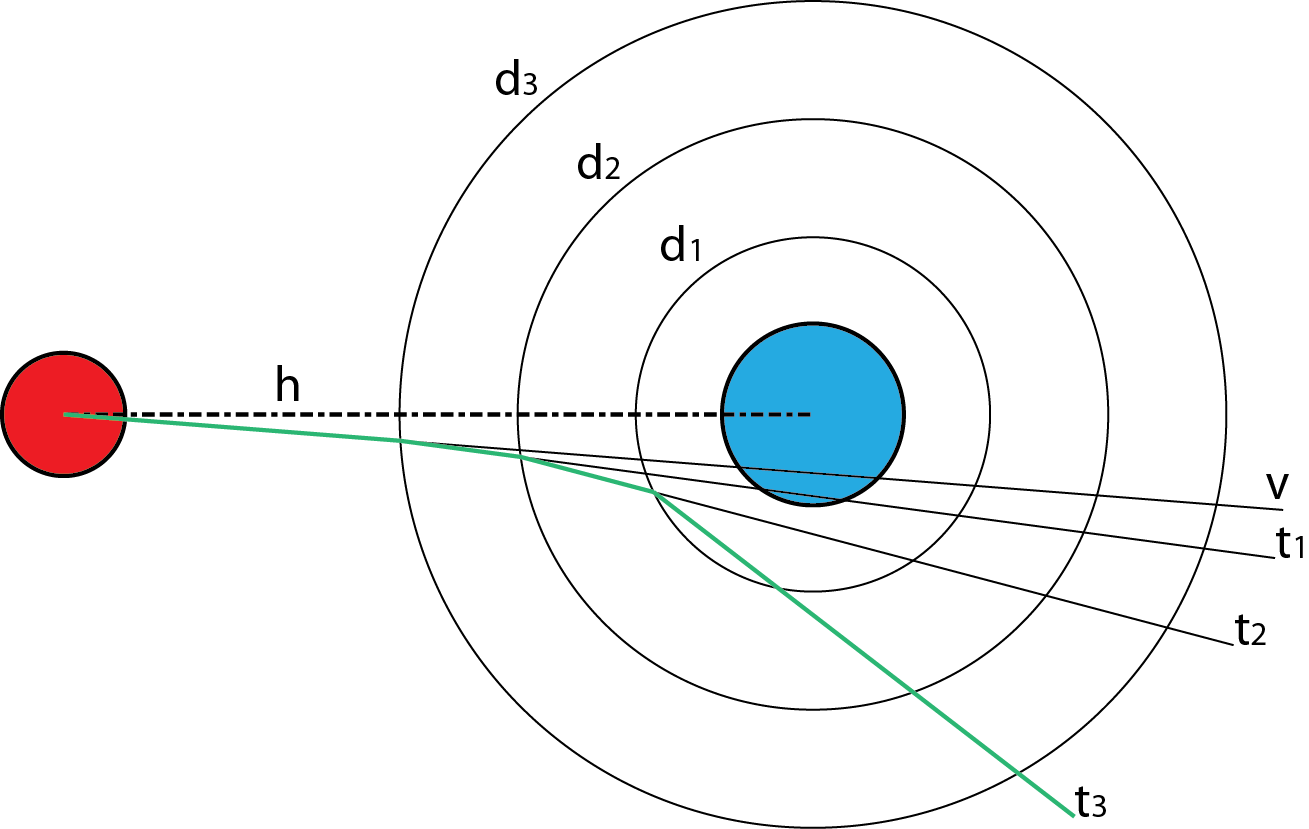
\includegraphics[width=0.8\textwidth]{images/AC02.png}
    \caption{Fuzzy System Based on Collision Distance}
    \label{fuzzy system based on collision distance}
  \end{center}
\end{figure}

\chapter{Examples}

\section{Field}

When you want to build an experiment, you need to create a new field. In this new field you can include all the objects you need in the package ``objects'' and the tools in he package ``tools''. The generic operations can be included into ``function'' class into ``tools'' package as static functions. The idea is not to have the same mathematic functions in the fields.

\section{Axis Field}

Here I have included a main axis reference.

\section{Grids Field}

Here I have included the main grid with the normal along the $Z$ axis.

\section{Collisions Field}

This is an experiment to create a system of robots and obstacles to try to avoid collisions among them as you can see in Figure \ref{collisions field}. Here I use the following classes:

\begin{description}
  \item[Wall ] This class allow us to create walls to define rooms where inside the robots are going to bounce.
  \item[Robot ] A class which defines a simple robot that mainly consists of a red cylinder.
  \item[Obstacle ] A class which defines a simple robot that mainly consists of a blue cylinder.
\end{description}

\begin{figure}[htbp]
  \begin{center}
    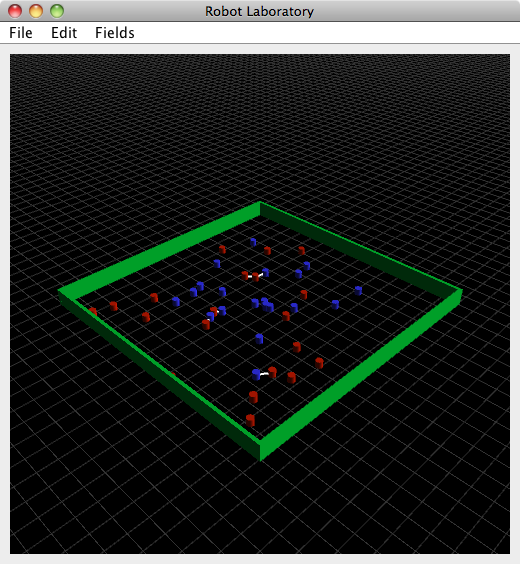
\includegraphics[width=0.5\textwidth]{images/CF.png}
    \caption{Collisions Field}
    \label{collisions field}
  \end{center}
\end{figure}

\newpage
\section{DHRobot Field}

This is a simple field to draw static robots with different configurations, based on Denavit-Hartenberg algorithms, as you can see in Figure \ref{static robots}.

\begin{figure}[htbp]
  \begin{center}
    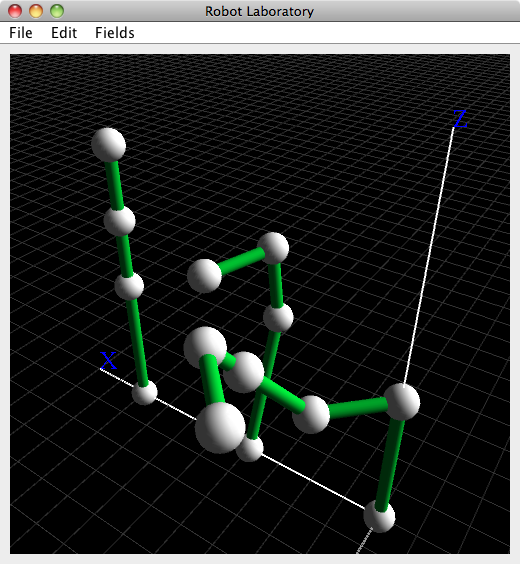
\includegraphics[width=0.5\textwidth]{images/SR.png}
    \caption{Static Robots}
    \label{static robots}
  \end{center}
\end{figure}

\newpage
\section{DHRobotB1 Field}

This is an example of a few robots dancing on the screen. I have used denavit-hartenberg normal robots and I have added a base to make them more visual. I want to test the arm manipulation capabilities of the DH algorithm, as you can see in Figure \ref{dancing dobots}.

\begin{figure}[htbp]
  \begin{center}
    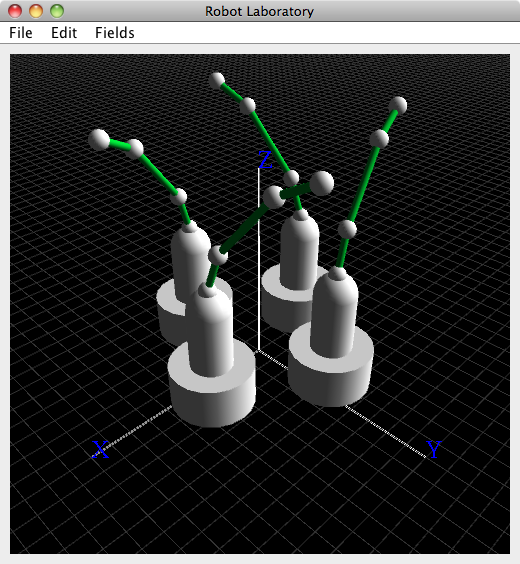
\includegraphics[width=0.5\textwidth]{images/DR.png}
    \caption{Dancing Robots}
    \label{dancing dobots}
  \end{center}
\end{figure}

\end{document}
